The first step in the TRITIUM design was to choose the fibre length and the fibre diameter ($1$ or $2~\mm$) for which the signal of tritium events is optimized. For a given active area, the longer the fibres, the smaller the number of photosensors needed. However, in long fibres photons are reflected on their boundaries many times before reaching the photosensors, which may produce a deterioration in the tritium signal. To determine the optimal fibre length, several simulations, described in section \ref{subsec:FiberLengthSimulation}, were carried out using Geant4 \cite{Geant4WebPage}. It was concluded that the optimal fibre length for measuring tritium in water is around $20~\cm$, which is the fibre length used in the TRITIUM prototypes developed at IFIC and for most of the characterization studies carried out in this thesis. As the manufacturer \cite{SaintGobain} delivers $1~\meter$ long fibres, an effective cleaving technique had to be developed with stringent requirements on the cleaving quality, since this greatly affects the transmission of photons and, consequently, the detection efficiency of the TRITIUM detector. The cleaving must be done perpendicular to the fibre axis and with small uncertainty in the cleaving position to enable optimal coupling of the fibre to the photosensor. It is also important that the fibre integrity be preserved, without cracks or deformations that may contribute to photon loss. 

Cleaving plastic fibres is a current challenge. There are many different techniques such as milling, laser cleaving, focused-ion-beam, blade cleaving, etc. The blade cleaving technique was chosen because of its mechanical simplicity and because, unlike other techniques, it preserves the integrity of plastic fibres. Many commercial devices based on blade cleaving, such as the one provided by Thorlabs with a diamond tipped blade \cite{DiamondThorlabs}, or guillotines designed for industrial fibre optics \cite{GuillotineIFO}, were tested in an comprehensive study with unsuccessful results \cite{TFGAlberto}. As it can be seen in Figure \ref{fig:BadCleavesOfFibers}, commercial techniques produce deformations, cracks and imperfections so they do not yield results with the quality standard required for the detector.
\begin{figure}
\centering
    \begin{subfigure}[b]{0.5\textwidth}
    \centering
    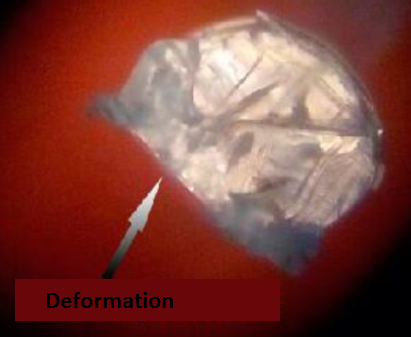
\includegraphics[width=\textwidth]{4ResearchAndDevelopments/41Fibers/DeformationFiberEnds.png}  
    \caption{\label{subfig:FiberEndDeformation}}
    \end{subfigure}
    \hfill
    \begin{subfigure}[b]{0.45\textwidth}
    \centering
    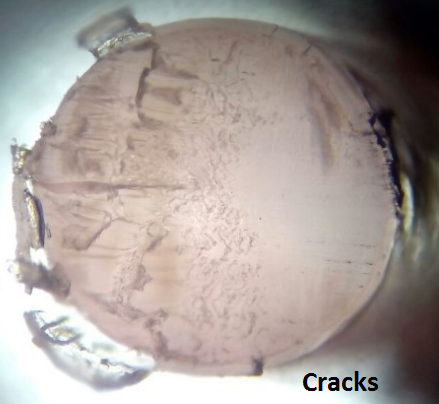
\includegraphics[width=\textwidth]{4ResearchAndDevelopments/41Fibers/CracksEndFibers.png}  
    \caption{\label{subfig:FiberEndCracks}}
    \end{subfigure}
 \caption{Results of using commercial techniques for cleaving the scintillating fibres a) Fibre end deformation b) Fibre end cracks. Pictures taken with a microscope PB 4161 from EUROMEX.}
 \label{fig:BadCleavesOfFibers}
\end{figure}
Because commercial devices are not suitable for polymer fibres, a cleaving device, shown in Figure \ref{fig:CleaveTRITIUMDevice}, was designed and built at IFIC laboratory.
\begin{figure}
\centering
    \begin{subfigure}[b]{0.5\textwidth}
    \centering
    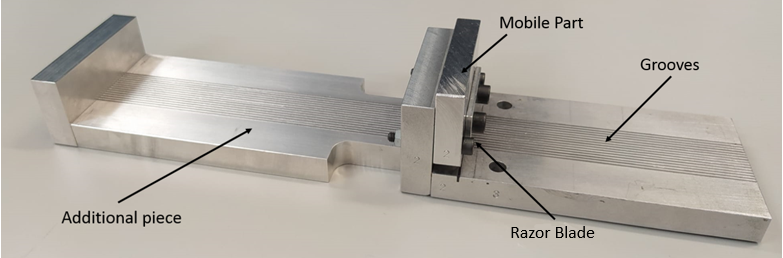
\includegraphics[width=\textwidth]{4ResearchAndDevelopments/41Fibers/CuttingDevice.png}  
    \caption{\label{subfig:CleaveTRITIUMDevice1}}
    \end{subfigure}
    \hfill
    \begin{subfigure}[b]{0.45\textwidth}
    \centering
    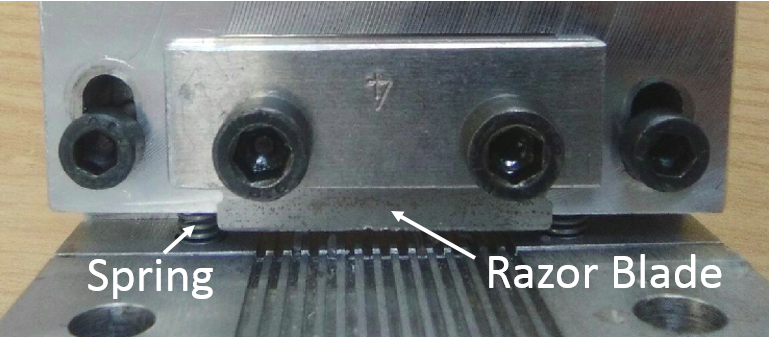
\includegraphics[width=\textwidth]{4ResearchAndDevelopments/41Fibers/Cleaving_machine_ZOOM.png}  
    \caption{\label{subfig:CleaveTRITIUMDeviceZOOM}}
    \end{subfigure}
 \caption{Plastic fibre cleaver developed in TRITIUM project. \label{fig:CleaveTRITIUMDevice}}
\end{figure}
This device consists of an aluminium plate endowed with fourteen grooves to accommodate the fibres. A thin razor blade attached to a mobile piece is used to cleave the fibres. The perpendicular cleave, which is one of the requirements, can be ensured since the moving piece to which the blade is attached is placed perpendicular to the fibre axis. The blade used is a typical commercial razor blade, of $0.1~\mm$ thickness, which is the thickness that gave the best results. The blade was positioned with a $5\degree$ inclination with respect to the horizontal axis since it was found in several studies that this helps to obtain a less aggressive and cleaner cleave \cite{AngleBlade, TemperatureBlade}. As it can be seen in Figure \ref{fig:CleavingFiberEnd}, the integrity of the fibre is preserved and no deformation is observed. However, it can be noticed some tears on the clad, but it is reported in section \ref{subsubsec:CharacterizationFibers} that these tears affect negligibly the photon collection. 

An additional parameter that could affect the cleaving quality of the fibre ends is the temperature of both fibre and blade. A study was carried out in which both were subject to different temperatures, from room temperature to $110\celsius$. No significant conclusions were obtained \cite{TFGAlberto}. Thus, the cleaving process was carried out at room temperature to make the cleaving process easier.

\begin{figure}[h]
\centering
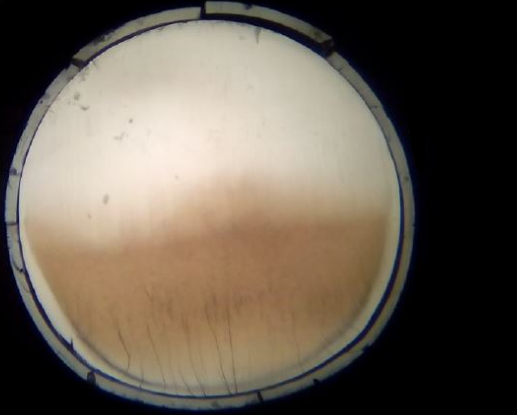
\includegraphics[scale=0.75]{4ResearchAndDevelopments/41Fibers/CutEndFiberGood.png}
\caption{Fibre end after cleaving process using the home-made cleaver. Pictures taken with the microscope PB 4161 from EUROMEX.\label{fig:CleavingFiberEnd}}
\end{figure}

A second L-shaped aluminium plate with grooves was attached to the first one (see Figure \ref{fig:CleaveTRITIUMDevice}) to set accurately the length of the fibres to $200~\mm$, with an uncertainty of $\pm 1~\mm$.